\documentclass[../PianodiProgetto.tex]{subfiles}

\begin{document}
	
	\chapter{Modello di sviluppo}
	
	Il modello di sviluppo adottato dal gruppo è il \glossario{modello incrementale}{modello incrementale}. Le motivazioni che hanno portato alla scelta di questo modello sono:
	\begin{itemize}
		\item Possibilità di suddividere il lavoro in più sottoattività sviluppate in modo parallelo. Questo permette maggior controllo sull’avanzamento del progetto;
		\item Lo sviluppo avviene per incrementi, dove ogni incremento rilascia parte delle funzionalità richieste;
		\item I requisiti vengono suddivisi in livelli di priorità. Quelli a priorità maggiore verranno soddisfatti con i primi incrementi, questo permette più attività di verifica e quindi maggiore stabilità ad ogni iterazione;
		\item I primi incrementi possono essere usati come prototipo per aiutare a definire i requisiti degli incrementi successivi;
		\item Minimizzare i rischi di ritardo rispetto ai tempi stabiliti in quanto i cicli hanno durata breve e sono precedentemente pianificati.
	\end{itemize}
	Alla fine della prima fase di codifica si avrà un prototipo funzionante con le implementazioni dei requisiti obbligatori. Tramite incrementi successivi verranno integrate le funzionalità opzionali e/o desiderabili.
	
	\chapter{Pianificazione}
	
	La pianificazione del lavoro è stata costruita sulla base delle scadenze elencate alla sezione 1.5 del seguente documento. In base ad esse, si è suddiviso lo sviluppo nei periodi seguenti:
	\begin{itemize}
		\item Analisi;
		\item Consolidamento dei requisiti;
		\item Consolidamento delle tecnologie;
		\item Progettazione e Codifica;
		\item Validazione e collaudo.
	\end{itemize}
	\newpage
	
	\section{Gestione delle scadenze temporali}
	
	Vista la presenza delle scadenze temporali definite nel PP, si necessita di un sistema di controllo efficiente dei tempi. Le procedure di controllo che verranno attuate per individuare e correggere eventuali errori sono descritte
	nelle NP. Nel tentativo di prevenire l'insorgenza di errori stessi, ogni attività svolta detiene un periodo iniziale di
	studio sull'argomento, che riduce la quantità di interventi correttivi a posteriori.
	
	\section{Gestione delle risorse}
	
	Il controllo eseguito per garantire il livello qualitativo di processi e prodotti necessita di risorse umane e tecnologiche. In relazione a questa attività, i ruoli di maggior rilievo sono il \textit{Responsabile} e il \textit{Verificatore}, che rispettivamente si occupano del controllo di qualità del processo e del prodotto risultante. Una descrizione dettagliata di tali ruoli è reperibile nel documento NP. 
	Le risorse tecnologiche comprendono tutti gli strumenti software e hardware che vengono utilizzati per attuare le procedure di verifica, automatizzate e non. Una descrizione dettagliata di tali risorse è reperibile nel documento NP. 
	
	\section{Analisi}
	Inizia con la formazione del gruppo e termina con la scadenza per la consegna della Revisione dei Requisiti.
	Durante questo periodo viene fatta un'analisi del capitolato scelto, in particolare vengono svolte le seguenti attività:
	\begin{itemize}
		\item \textbf{Individuazione delle norme:} vengono individuati gli strumenti e le norme relative ai vari processi per il corretto svolgimento del progetto;
		\item \textbf{Analisi dei capitolati:} in questa attività vengono studiati i vari capitolati, analizzando i vari pro e contro, scegliendo quale sviluppare;
		\item \textbf{Analisi dei Requisiti:} viene effettuata un'analisi approfondita dei requisiti del capitolato che il gruppo ha deciso di sviluppare;
		\item \textbf{Piano di Progetto:} viene scelto il modello di sviluppo e fatta la pianificazione per la realizzazione del progetto suddividendo le risorse disponibili, analizzando i vari rischi in cui si può incombere, realizzando infine il preventivo; 
		\item \textbf{Pianificazione della qualità:} attività in cui si individuano gli obiettivi di qualità che si vuole raggiungere.	
	\end{itemize}
	
	\subsection{Analisi - diagramma di Gantt}
	\begin{figure}[H]
		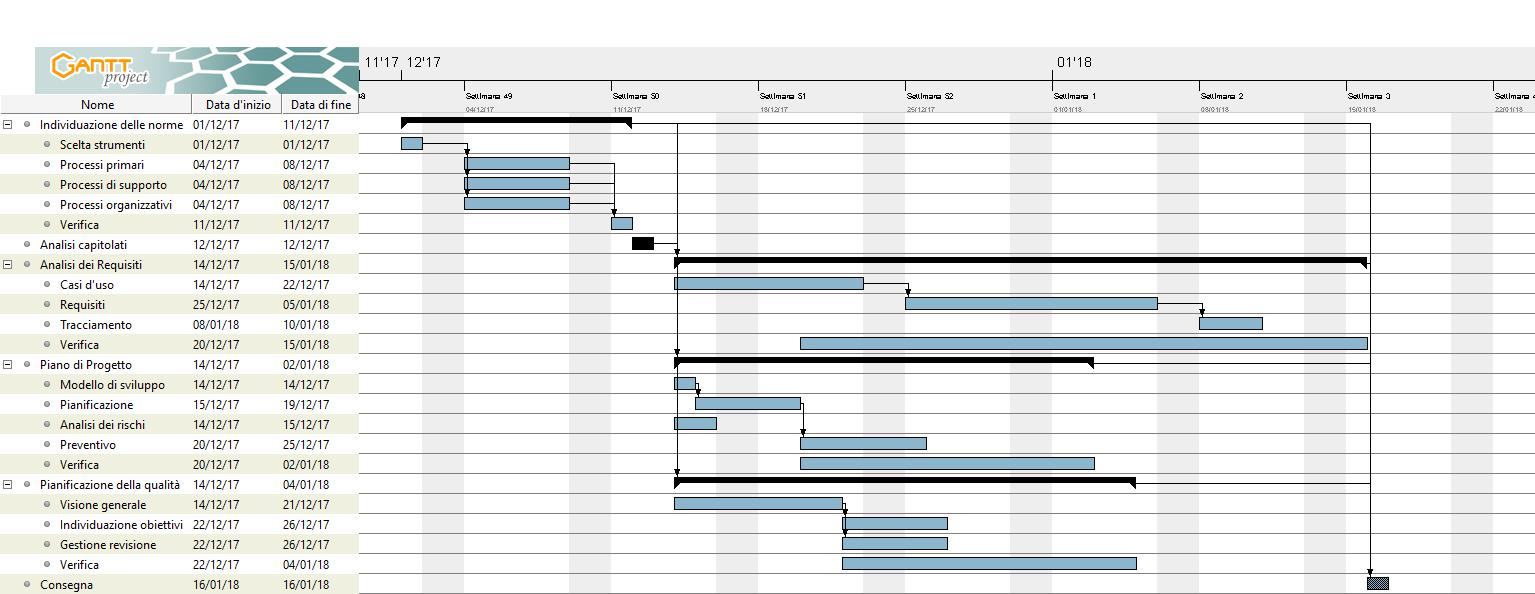
\includegraphics[width=1\linewidth]{pianificazione/AnalisiGantt.jpg}	
		\caption{Diagramma di Gantt di Analisi}\label{fig:1}	
	\end{figure}
	\newpage
		\section{Consolidamento dei requisiti} Inizia dopo la consegna dei documenti per la Revisione dei Requisiti e termina con la presentazione della Revisione dei Requisiti. Questo periodo consiste nel migliorare, consolidare ed eventualmente ampliare quanto fatto nell'Analisi dei Requisiti, in particolare i requisiti individuati.
	\subsection{Consolidamento dei requisiti - diagramma di Gantt}
	\begin{figure}[H]
		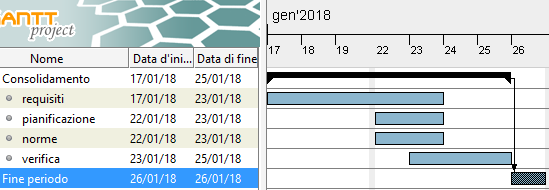
\includegraphics[width=\linewidth]{pianificazione/ConsolidamentoRequisitiGantt}	
		\caption{Diagramma di Gantt di Consolidamento dei requisiti}\label{fig:2}
	\end{figure}
	\newpage
	\section{Consolidamento delle tecnologie} Inizia dopo l'esito della Revisione dei Requisiti e termina con la consegna per la Revisione di Progettazione. In questo periodo viene svolto:

	\begin{itemize}	
		\item \textbf{Incremento e Verifica}: vengono incrementati e verificati, se necessario, i documenti già redatti, correggendo i difetti emersi nell'esito della Revisione dei Requisiti;
		\item \textbf{Consolidamento dei requisiti}: vengono ulteriormente affinati, ed eventualmente ampliati, i requisiti analizzati durante il periodo di Analisi secondo le indicazioni ricevute durante l'esito;
		\item \textbf{Technology Baseline:} vengono analizzate nel dettaglio le tecnologie scelte per il progetto individuando eventuali rischi delle stesse e mitigati mediante la realizzazione di un \glossario{Proof of Concept}{Proof of Concept} utile per il prodotto finale;
	\end{itemize}

	\subsection{Consolidamento delle tecnologie - diagramma di Gantt}
	\begin{figure}[H]
		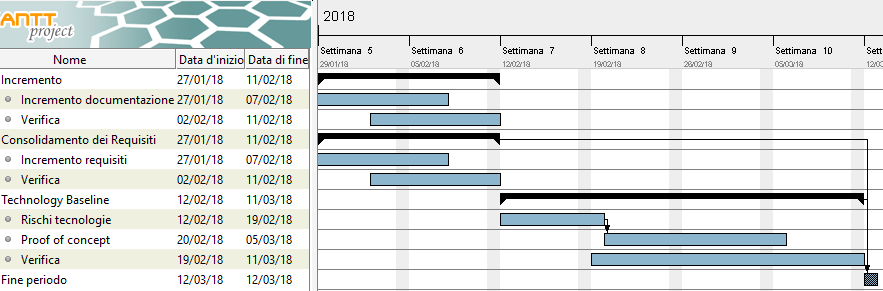
\includegraphics[width=\linewidth]{pianificazione/ConsolidamentoTecnologieGantt}	
		\caption{Diagramma di Gantt di Consolidamento delle tecnologie}\label{fig:3}
	\end{figure}
	\newpage
	\section{Progettazione e codifica}
	Inizia dopo la fine del periodo di Consolidamento e termina con la consegna per la Revisione di Qualifica. Durante questo periodo vengono svolte le seguenti attività:
	\begin{itemize}
		\item \textbf{Incremento e Verifica}: vengono incrementati e verificati, se necessario, i documenti già redatti, correggendo i difetti emersi nell'esito della Revisione di Progettazione;	
		\item \textbf{Progettazione:} vengono individuati i design pattern e costruita l'architettura del prodotto realizzando diagrammi di classi e di sequenza, il lavoro svolto rappresenterà la \glossario{Product Baseline}{Product Baseline};
		\item \textbf{Codifica:} consiste nella stesura del primo ciclo di codice per la creazione del prodotto che soddisfi i requisiti obbligatori individuati, aggiunti uno ad uno in modo incrementale.
	\end{itemize}
	\subsection{Progettazione e codifica - diagramma di Gantt}
	\begin{figure}[H]
		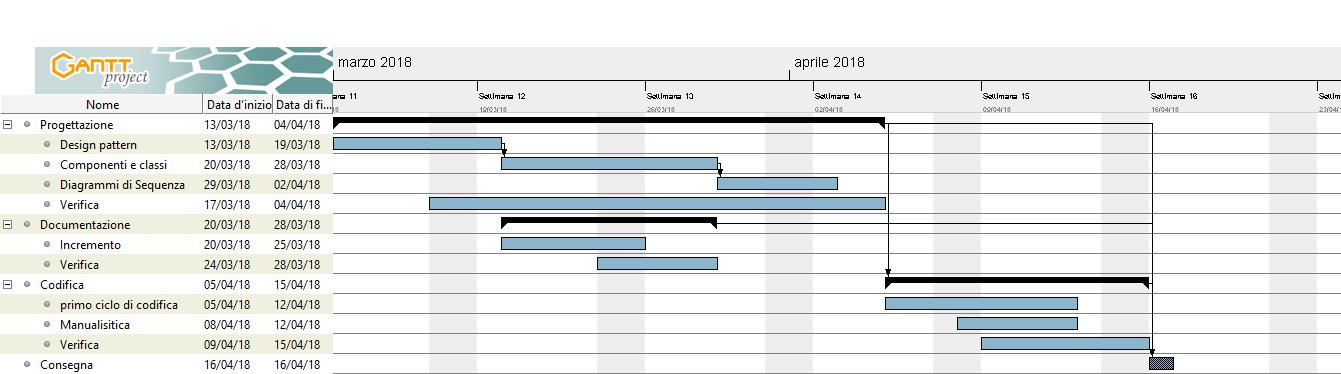
\includegraphics[width=\linewidth]{pianificazione/ProgettazioneCodificaGantt.jpg}	
		\caption{Diagramma di Gantt di Progettazione e Codifica}\label{fig:4}	
	\end{figure}
	\newpage
	\section{Validazione e collaudo}
	Inizia dopo la Revisione di Qualifica e termina con la Revisione di Accettazione del 14-05-2018. Durante questo periodo viene svolto:
	\begin{itemize}
		\item \textbf{Incremento e Verifica}: vengono incrementati e verificati, se necessario, i documenti già redatti e l'architettura del prodotto, correggendo i difetti emersi nell'esito della Revisione di Qualifica;
		\item \textbf{Codifica:} viene affinato il codice prodotto durante il primo ciclo, verificato, ed eventualmente incrementato con l'aggiunta di alcuni requisiti opzionali e/o desiderabili;		
		\item \textbf{Validazione e Collaudo:} viene verificata la conformità del prodotto rispetto ai requisiti, testandolo per assicurarsi il corretto funzionamento ed il raggiungimento di determinati vincoli qualificativi.
		 
	\end{itemize}
	\subsection{Validazione e collaudo - diagramma di Gantt}
	\begin{figure}[H]
		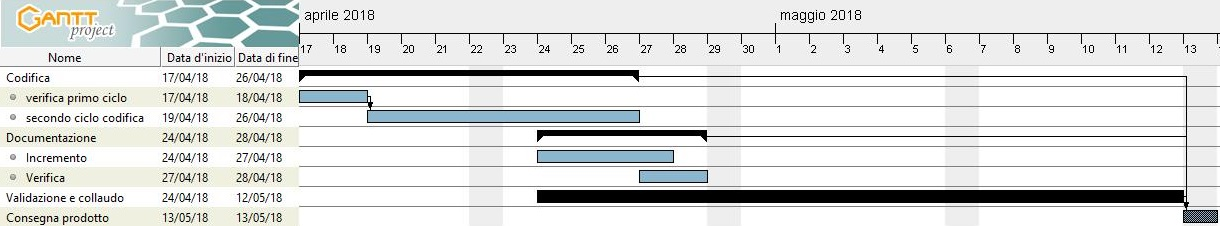
\includegraphics[width=\linewidth]{pianificazione/ValidazioneCollaudoGantt.jpg}	
		\caption{Diagramma di Gantt di Validazione e collaudo}\label{fig:5}	
	\end{figure}
\end{document}